\section{Results}
\label{sec:results}

We present results by hypothesis, then a format robustness check and a verifier sensitivity analysis.

\subsection{Instruction count (E1, H1)}

\para{{\bf How fast does compliance fall?}} \Figref{fig:e1} and \tabref{tab:e1} show that count has a strong effect at every model size. Mean per-instruction compliance falls from 83.4\% at $k=1$ to 70.3\% at $k=5$ and 59.1\% at $k=10$. The all-satisfied rate falls much further, to 37.0\% and 5.0\%. The best model, \qeight, satisfies all ten instructions in only 23.8\% of responses.

\begin{figure}[t]
\centering
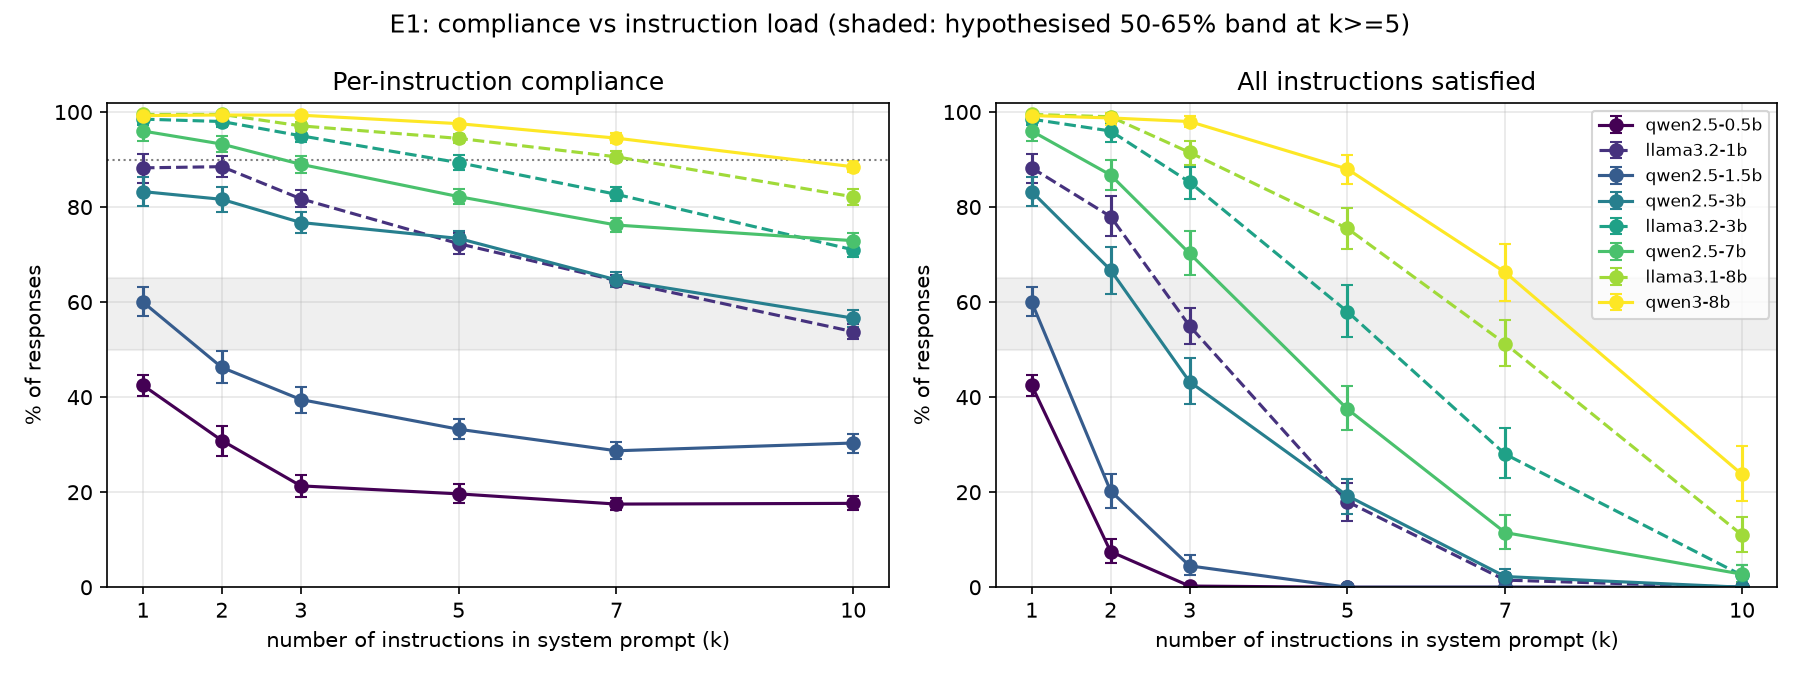
\includegraphics[width=0.95\linewidth]{figures/e1_load_curve.png}
\caption{Compliance against instruction count. \figleft Per-instruction compliance declines roughly linearly for most models, with a floor near 18\% for \qhalf. \figright The all-satisfied rate collapses, and no model exceeds 24\% at $k=10$. Shaded band: the hypothesized 50--65\% range at $k \geq 5$. Error bars: 95\% CIs.}
\label{fig:e1}
\end{figure}

\para{H1 is partially supported.} Single-instruction compliance exceeds 90\% for only 4 of 8 models. The small Qwen2.5 models often fail even one instruction (\qhalf 42.5\%, \qone 60.0\%). With $k \geq 5$, per-instruction compliance ranges from 18\% to 92\% depending on the model. The hypothesized 50--65\% band fits the mid-size models (\lone 61\%, \qthree 63\%) and the $k=10$ cross-model mean, but it does not fit the strongest models (88--92\%) or the weakest (18--30\%).

\para{Load does not hit all instructions equally.} \Tabref{tab:perinstruction} shows that among capable models, \ins{P_name} falls by 47\pp from $k=1$ to $k=10$, while \ins{L_max} falls by 6\pp. \ins{S_nocomma} even rises slightly, from 86.2\% to 90.7\%, because bullets, titles, and word limits shorten answers.

\begin{table}[t]
\centering
\caption{E1: per-instruction compliance (\%), with all-satisfied rate in parentheses. Bootstrap 95\% CI half-widths are about 3\pp or less. Best result per column in \textbf{bold}.}
\label{tab:e1}
\begin{tabular}{@{}lcccccc@{}}
\toprule
\textbf{Model} & $k=1$ & $k=2$ & $k=3$ & $k=5$ & $k=7$ & $k=10$ \\
\midrule
\qhalf & 42.5 & 30.9 (7.5) & 21.3 (0.2) & 19.6 (0.0) & 17.5 (0.0) & 17.6 (0.0) \\
\lone & 88.2 & 88.5 (78.0) & 81.8 (55.0) & 72.3 (18.0) & 64.5 (1.5) & 53.8 (0.0) \\
\qone & 60.0 & 46.2 (20.2) & 39.5 (4.5) & 33.2 (0.0) & 28.7 (0.0) & 30.4 (0.0) \\
\qthree & 83.2 & 81.6 (66.8) & 76.8 (43.2) & 73.4 (19.2) & 64.7 (2.2) & 56.6 (0.0) \\
\lthree & 98.5 & 98.0 (96.0) & 95.0 (85.2) & 89.4 (58.0) & 82.7 (28.0) & 71.0 (2.5) \\
\qseven & 96.0 & 93.2 (86.8) & 89.0 (70.2) & 82.2 (37.5) & 76.2 (11.5) & 72.9 (2.8) \\
\leight & \textbf{99.5} & \textbf{99.5} (\textbf{99.0}) & 97.1 (91.5) & 94.4 (75.5) & 90.6 (51.2) & 82.2 (11.0) \\
\qeight & 99.2 & 99.4 (98.8) & \textbf{99.3} (\textbf{98.0}) & \textbf{97.6} (\textbf{88.0}) & \textbf{94.5} (\textbf{66.2}) & \textbf{88.5} (\textbf{23.8}) \\
\midrule
Mean & 83.4 & 79.7 (69.1) & 75.0 (56.0) & 70.3 (37.0) & 64.9 (20.1) & 59.1 (5.0) \\
\bottomrule
\end{tabular}
\end{table}

\begin{table}[t]
\centering
\caption{E1 compliance (\%) by instruction, averaged over the six capable models. Name and bullet compliance fall steeply, while the word limit and no-comma rules barely move.}
\label{tab:perinstruction}
\resizebox{\textwidth}{!}{%
\begin{tabular}{@{}lcccccccccc@{}}
\toprule
& \ins{F_title} & \ins{F_bullets} & \ins{F_end} & \ins{L_max} & \ins{P_ahoy} & \ins{P_name} & \ins{P_matey} & \ins{S_lower} & \ins{S_nocomma} & \ins{S_keyword} \\
\midrule
$k=1$ & 97.5 & 95.0 & 91.2 & 99.6 & 100.0 & 93.3 & 100.0 & 89.2 & 86.2 & 89.2 \\
$k=5$ & 83.8 & 82.3 & 74.8 & 95.6 & 83.5 & 79.0 & 92.0 & 84.6 & 93.4 & 80.7 \\
$k=10$ & 67.7 & 57.9 & 57.5 & 93.7 & 70.2 & 45.9 & 90.5 & 68.1 & 90.7 & 66.1 \\
\bottomrule
\end{tabular}}
\end{table}


\subsection{Pairwise interference (E2, H2)}

\para{{\bf Do format and length rules suppress persona and style rules?}} \Tabref{tab:e2} shows that the direction holds for some models, but the hypothesized size does not hold in general. Persona and style instructions lose more next to a format or length partner than next to a persona or style partner in 4 of 8 models, with an extra drop of 5--12\pp. Drops of about 20\pp appear only in the two smallest Qwen models, and in those models persona and style partners also cause drops (\qhalf $-$16.9\pp). \lthree, \leight, and \qeight show no effect.

\begin{table}[t]
\centering
\caption{E2: change in persona/style (P/S) compliance relative to the same instruction alone, by partner group (pp). * marks Holm-adjusted $p<.05$. The contrast is the extra drop from a format/length (F/L) partner; \textbf{bold} contrasts have a 95\% CI that excludes 0.}
\label{tab:e2}
\begin{tabular}{@{}lccc@{}}
\toprule
\textbf{Model} & \textbf{F/L partner} & \textbf{P/S partner} & \textbf{Contrast (F/L $-$ P/S) [95\% CI]} \\
\midrule
\qhalf & $-$21.6* & $-$16.9* & \textbf{$-$4.7} [$-$9.1, $-$0.5] \\
\lone & $-$5.7 & +2.1 & \textbf{$-$7.8} [$-$11.4, $-$4.1] \\
\qone & $-$19.5* & $-$7.3 & \textbf{$-$12.2} [$-$17.6, $-$7.2] \\
\qthree & $-$3.4 & $-$0.8 & $-$2.6 [$-$7.6, 2.9] \\
\lthree & $-$0.3 & +0.2 & $-$0.5 [$-$2.4, 1.4] \\
\qseven & $-$6.2 & $-$1.5 & \textbf{$-$4.8} [$-$8.3, $-$1.1] \\
\leight & +1.0 & +0.4 & +0.6 [$-$0.5, 2.1] \\
\qeight & 0.0 & +0.8 & $-$0.8 [$-$2.0, 0.2] \\
\bottomrule
\end{tabular}
\end{table}


\para{Interference is specific, not categorical.} \Figref{fig:e2} shows the full matrix for the six models with single-instruction compliance of at least 80\%. Large cells include \partnerarrow{F_bullets}{F_end} ($-$30\pp), \partnerarrow{F_bullets}{S_keyword} ($-$20\pp), \partnerarrow{S_nocomma}{F_end} ($-$15\pp), \partnerarrow{F_bullets}{P_name}, \partnerarrow{L_max}{S_keyword}, and \partnerarrow{P_matey}{P_name} (each $-$12\pp), and \partnerarrow{P_ahoy}{P_name} ($-$11\pp). The strongest effect is format on format, which H2 does not anticipate. \qthree shows it most clearly: format and length targets with a format or length partner drop 19\pp (Holm-adjusted $p<.001$). The \partnerarrow{F_title}{P_ahoy} cell, which appears as $-$12\pp in \figref{fig:e2}, is mostly a verifier artifact (\secref{sec:sensitivity}).

\begin{figure}[t]
\centering
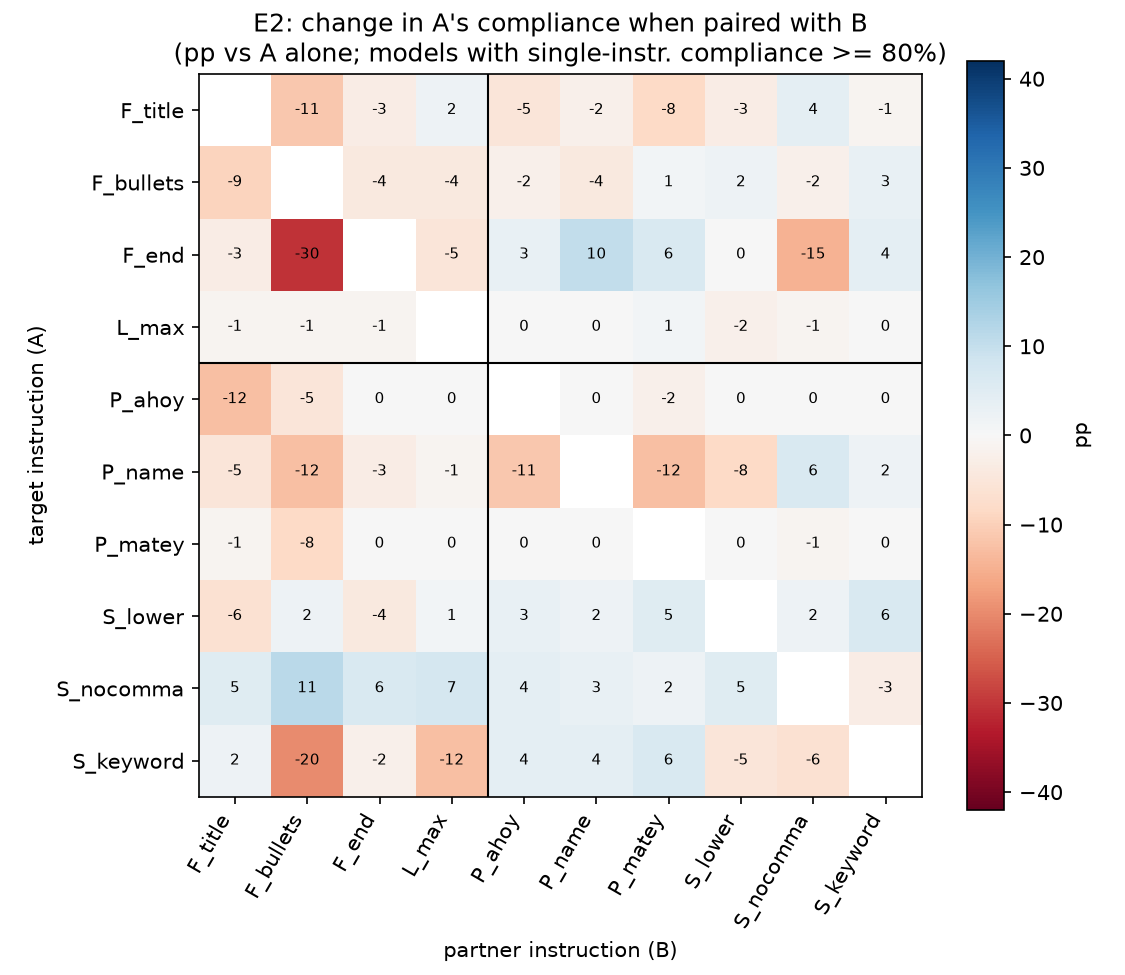
\includegraphics[width=0.62\linewidth]{figures/e2_interference_matrix_capable.png}
\caption{Change in target A's compliance when paired with partner B, relative to A alone on the same task (pp), averaged over the six capable models. Each model contributes 16 responses per cell. Large drops sit in a few cells, mainly the \ins{F_bullets} column. The \ins{S_nocomma} row shows facilitation. The \ins{F_title}/\ins{P_ahoy} cell is inflated by the verifier issue in \secref{sec:sensitivity}.}
\label{fig:e2}
\end{figure}

\para{Large cells vary by model.} These means hide strong differences. \partnerarrow{F_bullets}{F_end} ranges from $-$69\pp for \lthree to 0\pp for \qeight. \partnerarrow{S_nocomma}{F_end} comes entirely from two Llama models (\lthree $-$69\pp, \lone $-$19\pp), and the other four models show 0\pp. \partnerarrow{P_ahoy}{P_name} comes mainly from \qthree ($-$56\pp). With 16 responses per model and cell, these per-model values are noisy.

\para{{\bf Why do these pairs interfere?}} Failure inspection points to \emph{layout capture}. With ``exactly 3 bullets'', models tend to output only the bullets and drop whatever must live outside them. In the \partnerarrow{F_bullets}{F_end} cell, none of the 40 failures among the 96 capable-model responses contains the closing phrase at all. Similarly, a response that opens with ``Ahoy! Ahoy there, matey!'' satisfies the opening but can crowd out the self-introduction.

\para{Some pairs help.} \ins{S_nocomma} gains 5--11\pp next to \ins{F_title}, \ins{F_bullets}, \ins{F_end}, and \ins{L_max}, because structured or shorter answers contain fewer commas.

\subsection{Position (E3, H3)}

\para{{\bf Does the last instruction win?}} H3 is not supported in magnitude. \Tabref{tab:e3} shows a small overall recency advantage of +1.7\pp [0.8, 2.7], and no model reaches the hypothesized +15\pp. Only two models show a Holm-significant effect: \qthree (+8.2\pp) and \qeight (+5.2\pp, failures fall from 7\% to 2\%). Llama models show no recency benefit. The random orders in E1 agree: last-third minus first-third compliance is +5.5\pp for \qeight and +4.9\pp for \qthree, and it ranges from $-$3.1\pp to +1.3\pp for Llama models.

\begin{table}[t]
\centering
\caption{E3: target compliance (\%) by position among 5 instructions. $p$ values are Holm-adjusted across models; the pooled row is unadjusted. \textbf{Bold} marks $p<.05$.}
\label{tab:e3}
\begin{tabular}{@{}lcccc@{}}
\toprule
\textbf{Model} & \textbf{First} & \textbf{Last} & \textbf{Last $-$ first [95\% CI]} & $p$ \\
\midrule
\qhalf & 20.2 & 23.2 & +3.0 [0.7, 5.5] & .20 \\
\lone & 77.0 & 73.2 & $-$3.8 [$-$8.0, 0.8] & .50 \\
\qone & 34.0 & 32.0 & $-$2.0 [$-$6.2, 2.0] & 1.0 \\
\qthree & 65.8 & 74.0 & \textbf{+8.2} [4.2, 12.5] & .005 \\
\lthree & 89.2 & 88.0 & $-$1.2 [$-$4.2, 2.0] & 1.0 \\
\qseven & 80.8 & 84.0 & +3.2 [0.0, 6.5] & .45 \\
\leight & 94.5 & 95.0 & +0.5 [$-$1.2, 2.2] & 1.0 \\
\qeight & 93.0 & 98.2 & \textbf{+5.2} [3.0, 7.5] & $<$.001 \\
\midrule
All models & 69.3 & 71.0 & \textbf{+1.7} [0.8, 2.7] & .002 \\
\bottomrule
\end{tabular}
\end{table}


\subsection{Repetition (E4, H4)}

\para{{\bf Is repetition a free improvement?}} H4 holds in direction but not in magnitude. \Tabref{tab:e4} shows that repeating an instruction raises its compliance by +3.3\pp. The largest gains are in \qone (+6.8\pp) and \qseven (+6.0\pp), and no model reaches +10\pp. The other instructions lose 0.9\pp, far below the hypothesized 5--8\pp. A neutral filler line in the same slot causes the same loss, and repeat and filler do not differ for the other instructions (+0.1\pp [$-$0.5, 0.6]). So the collateral cost comes from a longer prompt, not from repetition. \Figref{fig:e3e4} shows per-model results.

\begin{table}[t]
\centering
\caption{E4: repetition effects in pp [95\% CI], pooled over 8 models (3,200 paired items per condition).}
\label{tab:e4}
\begin{tabular}{@{}lccc@{}}
\toprule
\textbf{Measure} & \textbf{Repeat $-$ base} & \textbf{Repeat $-$ filler} & \textbf{Filler $-$ base} \\
\midrule
Repeated instruction & \textbf{+3.3} [2.2, 4.5] & \textbf{+4.4} [3.2, 5.5] & $-$1.0 [$-$2.1, 0.0] \\
Other 4 instructions & \textbf{$-$0.9} [$-$1.4, $-$0.3] & +0.1 [$-$0.5, 0.6] & \textbf{$-$0.9} [$-$1.4, $-$0.5] \\
\bottomrule
\end{tabular}
\end{table}


\begin{figure}[t]
\centering
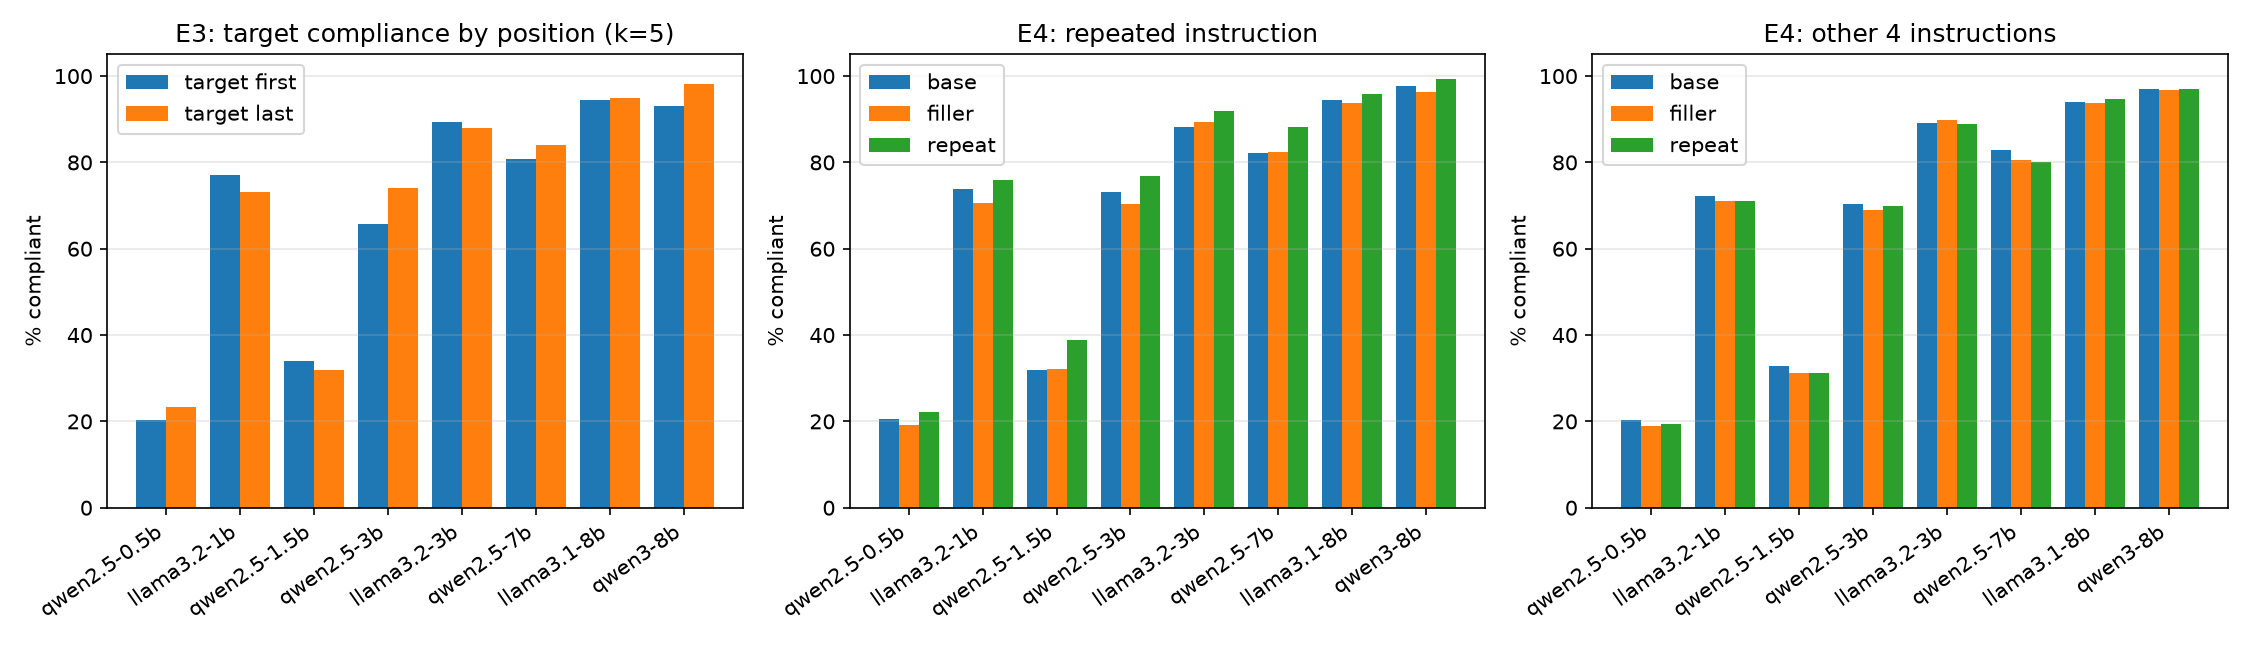
\includegraphics[width=0.95\linewidth]{figures/e3_e4_position_repetition.png}
\caption{\figleft E3: target compliance when placed first or last. \figcenter E4: compliance of the repeated instruction under base, filler, and repeat conditions. \figright E4: compliance of the other 4 instructions. Differences between conditions are small compared with differences between models.}
\label{fig:e3e4}
\end{figure}

\subsection{Model size (H5)}

\para{{\bf Do smaller models decay faster?}} The answer depends on the scale (\tabref{tab:h5}). Relative to their own baseline, smaller models lose much more: \qhalf loses 57\% of its compliance, while \qeight loses 7\% (Spearman $\rho=-0.95$, $p<.001$). In absolute pp per added instruction there is no size trend ($\rho=0.07$, $p=.87$), because floor models have little left to lose and ceiling models lose slowly at first. On the logit scale, the trend points the other way, but it is not significant across 8 models ($\rho=-0.64$, $p=.09$): \qeight multiplies its odds by 0.65 per added instruction, and \qhalf by 0.83. Family matters too, since Llama models have steeper logit slopes than Qwen2.5 models of similar size.

\begin{table}[t]
\centering
\caption{H5: decay by model size. The slope is pp per added instruction, the relative drop compares $k=1$ with $k \geq 5$, and the logit slope comes from the logistic GLM (95\% CIs in brackets). Models are sorted by size. Shallowest slope and smallest drop in \textbf{bold}.}
\label{tab:h5}
\resizebox{\textwidth}{!}{%
\begin{tabular}{@{}lcccc@{}}
\toprule
\textbf{Model} & \textbf{Params (B)} & \textbf{Slope (pp)} & \textbf{Relative drop} & \textbf{Logit slope} \\
\midrule
\qhalf & 0.5 & \textbf{$-$1.30} [$-$1.48, $-$1.14] & 57\% & $-$0.18 [$-$0.21, $-$0.16] \\
\lone & 1.2 & $-$3.99 [$-$4.21, $-$3.75] & 30\% & $-$0.24 [$-$0.26, $-$0.23] \\
\qone & 1.5 & $-$1.80 [$-$2.15, $-$1.46] & 49\% & \textbf{$-$0.13} [$-$0.16, $-$0.11] \\
\qthree & 3.1 & $-$3.05 [$-$3.35, $-$2.76] & 24\% & $-$0.18 [$-$0.20, $-$0.16] \\
\lthree & 3.2 & $-$3.36 [$-$3.56, $-$3.14] & 20\% & $-$0.35 [$-$0.37, $-$0.33] \\
\qseven & 7.6 & $-$2.38 [$-$2.62, $-$2.12] & 21\% & $-$0.20 [$-$0.23, $-$0.18] \\
\leight & 8.0 & $-$2.15 [$-$2.40, $-$1.89] & 12\% & $-$0.34 [$-$0.38, $-$0.30] \\
\qeight & 8.2 & $-$1.47 [$-$1.63, $-$1.30] & \textbf{7\%} & $-$0.44 [$-$0.49, $-$0.39] \\
\bottomrule
\end{tabular}}
\end{table}


\subsection{Robustness: numbered lists}

We rerun E1 and E3 with numbered instructions on four models. Load curves barely change. Compliance at $k=1/5/10$ moves from 98.5/89.4/71.0 to 98.5/89.0/71.1 for \lthree, from 83.2/73.4/56.6 to 86.2/70.3/53.4 for \qthree, and from 99.2/97.6/88.5 to 99.8/98.0/92.6 for \qeight. Numbering helps \qeight by 4\pp at $k=10$ and hurts \qthree by 3\pp. Position signs are unchanged: \qthree +7.0\pp, \qeight +3.0\pp, \lthree $-$3.0\pp, and \qone $-$3.8\pp.

\subsection{Verifier sensitivity}
\label{sec:sensitivity}

\Tabref{tab:sensitivity} reports the full analysis rerun with the corrected \ins{P_ahoy} check from \secref{sec:method}. Our main conclusions hold: count stays dominant, position and repetition stay small, and the Spearman results for H5 are unchanged to the reported precision. The same four models keep a contrast that excludes 0 in \tabref{tab:e2}. Two details change. First, the \partnerarrow{F_title}{P_ahoy} interference is mostly an artifact: it shrinks from $-$12.5\pp to $-$3.1\pp, and \qthree rises from 50\% to 100\% in this cell, so we do not count it as evidence of layout capture. Second, the \qthree recency effect shrinks to +6.5\pp, although it stays significant.

\begin{table}[t]
\centering
\caption{Effect of the corrected \ins{P_ahoy} verifier on the results that change most. Other pooled results move by less than 1\pp. Across E1, the largest single-model shifts are 1.7\pp in compliance and 4.3\pp in the all-satisfied rate, both at $k=5$ and in the models listed here.}
\label{tab:sensitivity}
\begin{tabular}{@{}llcc@{}}
\toprule
\textbf{Experiment} & \textbf{Result} & \textbf{Original} & \textbf{Corrected} \\
\midrule
E1 & Mean compliance, $k=5$ / $k=10$ & 70.3 / 59.1 & 70.7 / 59.3 \\
E1 & Mean all-satisfied rate, $k=5$ / $k=10$ & 37.0 / 5.0 & 38.2 / 5.0 \\
E1 & \qthree all-satisfied rate, $k=5$ & 19.2 & 23.5 \\
E1 & \lone all-satisfied rate, $k=5$ & 18.0 & 22.2 \\
E2 & \partnerarrow{F_title}{P_ahoy}, capable models (pp) & $-$12.5 & $-$3.1 \\
E2 & \qthree F/L $-$ P/S contrast (pp) & $-$2.6 & $-$0.5 \\
E3 & All models, last $-$ first (pp) & +1.7 ($p=.002$) & +1.4 ($p=.009$) \\
E3 & \qthree, last $-$ first (pp) & +8.2 ($p=.005$) & +6.5 ($p=.035$) \\
E4 & Repeated instruction, repeat $-$ base (pp) & +3.3 & +3.5 \\
E4 & Repeated instruction, filler $-$ base (pp) & $-$1.0 & $-$0.8 \\
\bottomrule
\end{tabular}
\end{table}

